% This example is meant to be compiled with lualatex or xelatex
% The theme itself also supports pdflatex
\PassOptionsToPackage{unicode}{hyperref}
\documentclass[aspectratio=1610, 9pt]{beamer}

% Load packages you need here
\usepackage{polyglossia}
\setmainlanguage{german}

\usepackage{csquotes}


\usepackage{amsmath}
\usepackage{amssymb}
\usepackage{mathtools}

\usepackage{hyperref}
\usepackage{bookmark}

\usepackage{xfrac}
\usepackage[shortcuts]{extdash}

\usepackage[
  backend=biber,
]{biblatex}
% Quellendatenbank
\addbibresource{lit.bib}

\usepackage[
  locale=DE,                   % deutsche Einstellungen
  separate-uncertainty=true,   % immer Fehler mit \pm
  per-mode=symbol-or-fraction, % / in inline math, fraction in display math
]{siunitx}

\usepackage{svrsymbols}
\usepackage{cancel}

% \AtBeginSection[]{
  % \frame{
    % \frametitle{Inhaltsverzeichnis}
      % \tableofcontents[currentsection]
  % }
% }

% load the theme after all packages

\usetheme[
  showtotalframes, % show total number of frames in the footline
]{tudo}

% Put settings here, like
\unimathsetup{
  math-style=ISO,
  bold-style=ISO,
  nabla=upright,
  partial=upright,
  mathrm=sym,
}

\title{W-Massenmessung}
\author[Julia ~Sobolewski]{Julia Sobolewski}
\institute[Fakultät Physik]{Fakultät Physik}
\titlegraphic{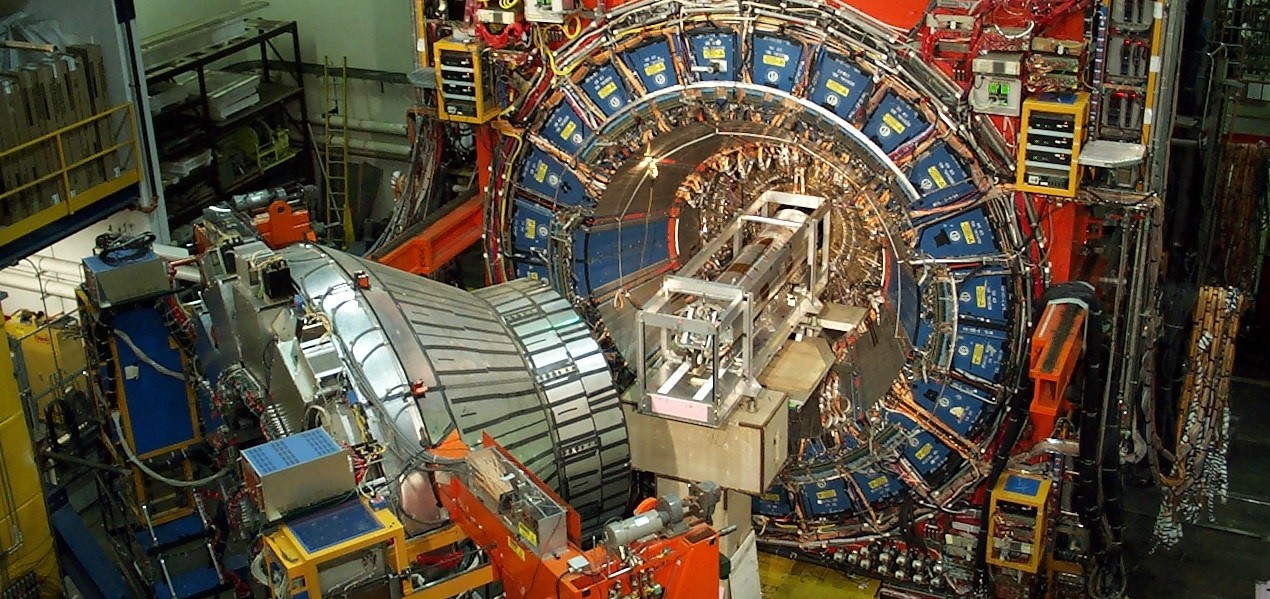
\includegraphics[width=0.7\textwidth]{images/cdf.jpg}}


\begin{document}

\maketitle

\begin{frame}[allowframebreaks]{Inhaltsverzeichnis}
  \tableofcontents
\end{frame}

\section{Einleitung}

\subsection{Was sind W-Bosonen?}

\begin{frame}{Was sind W-Bosonen?}
  \begin{columns}
    \begin{column}{0.4\textwidth}
      \begin{figure}
        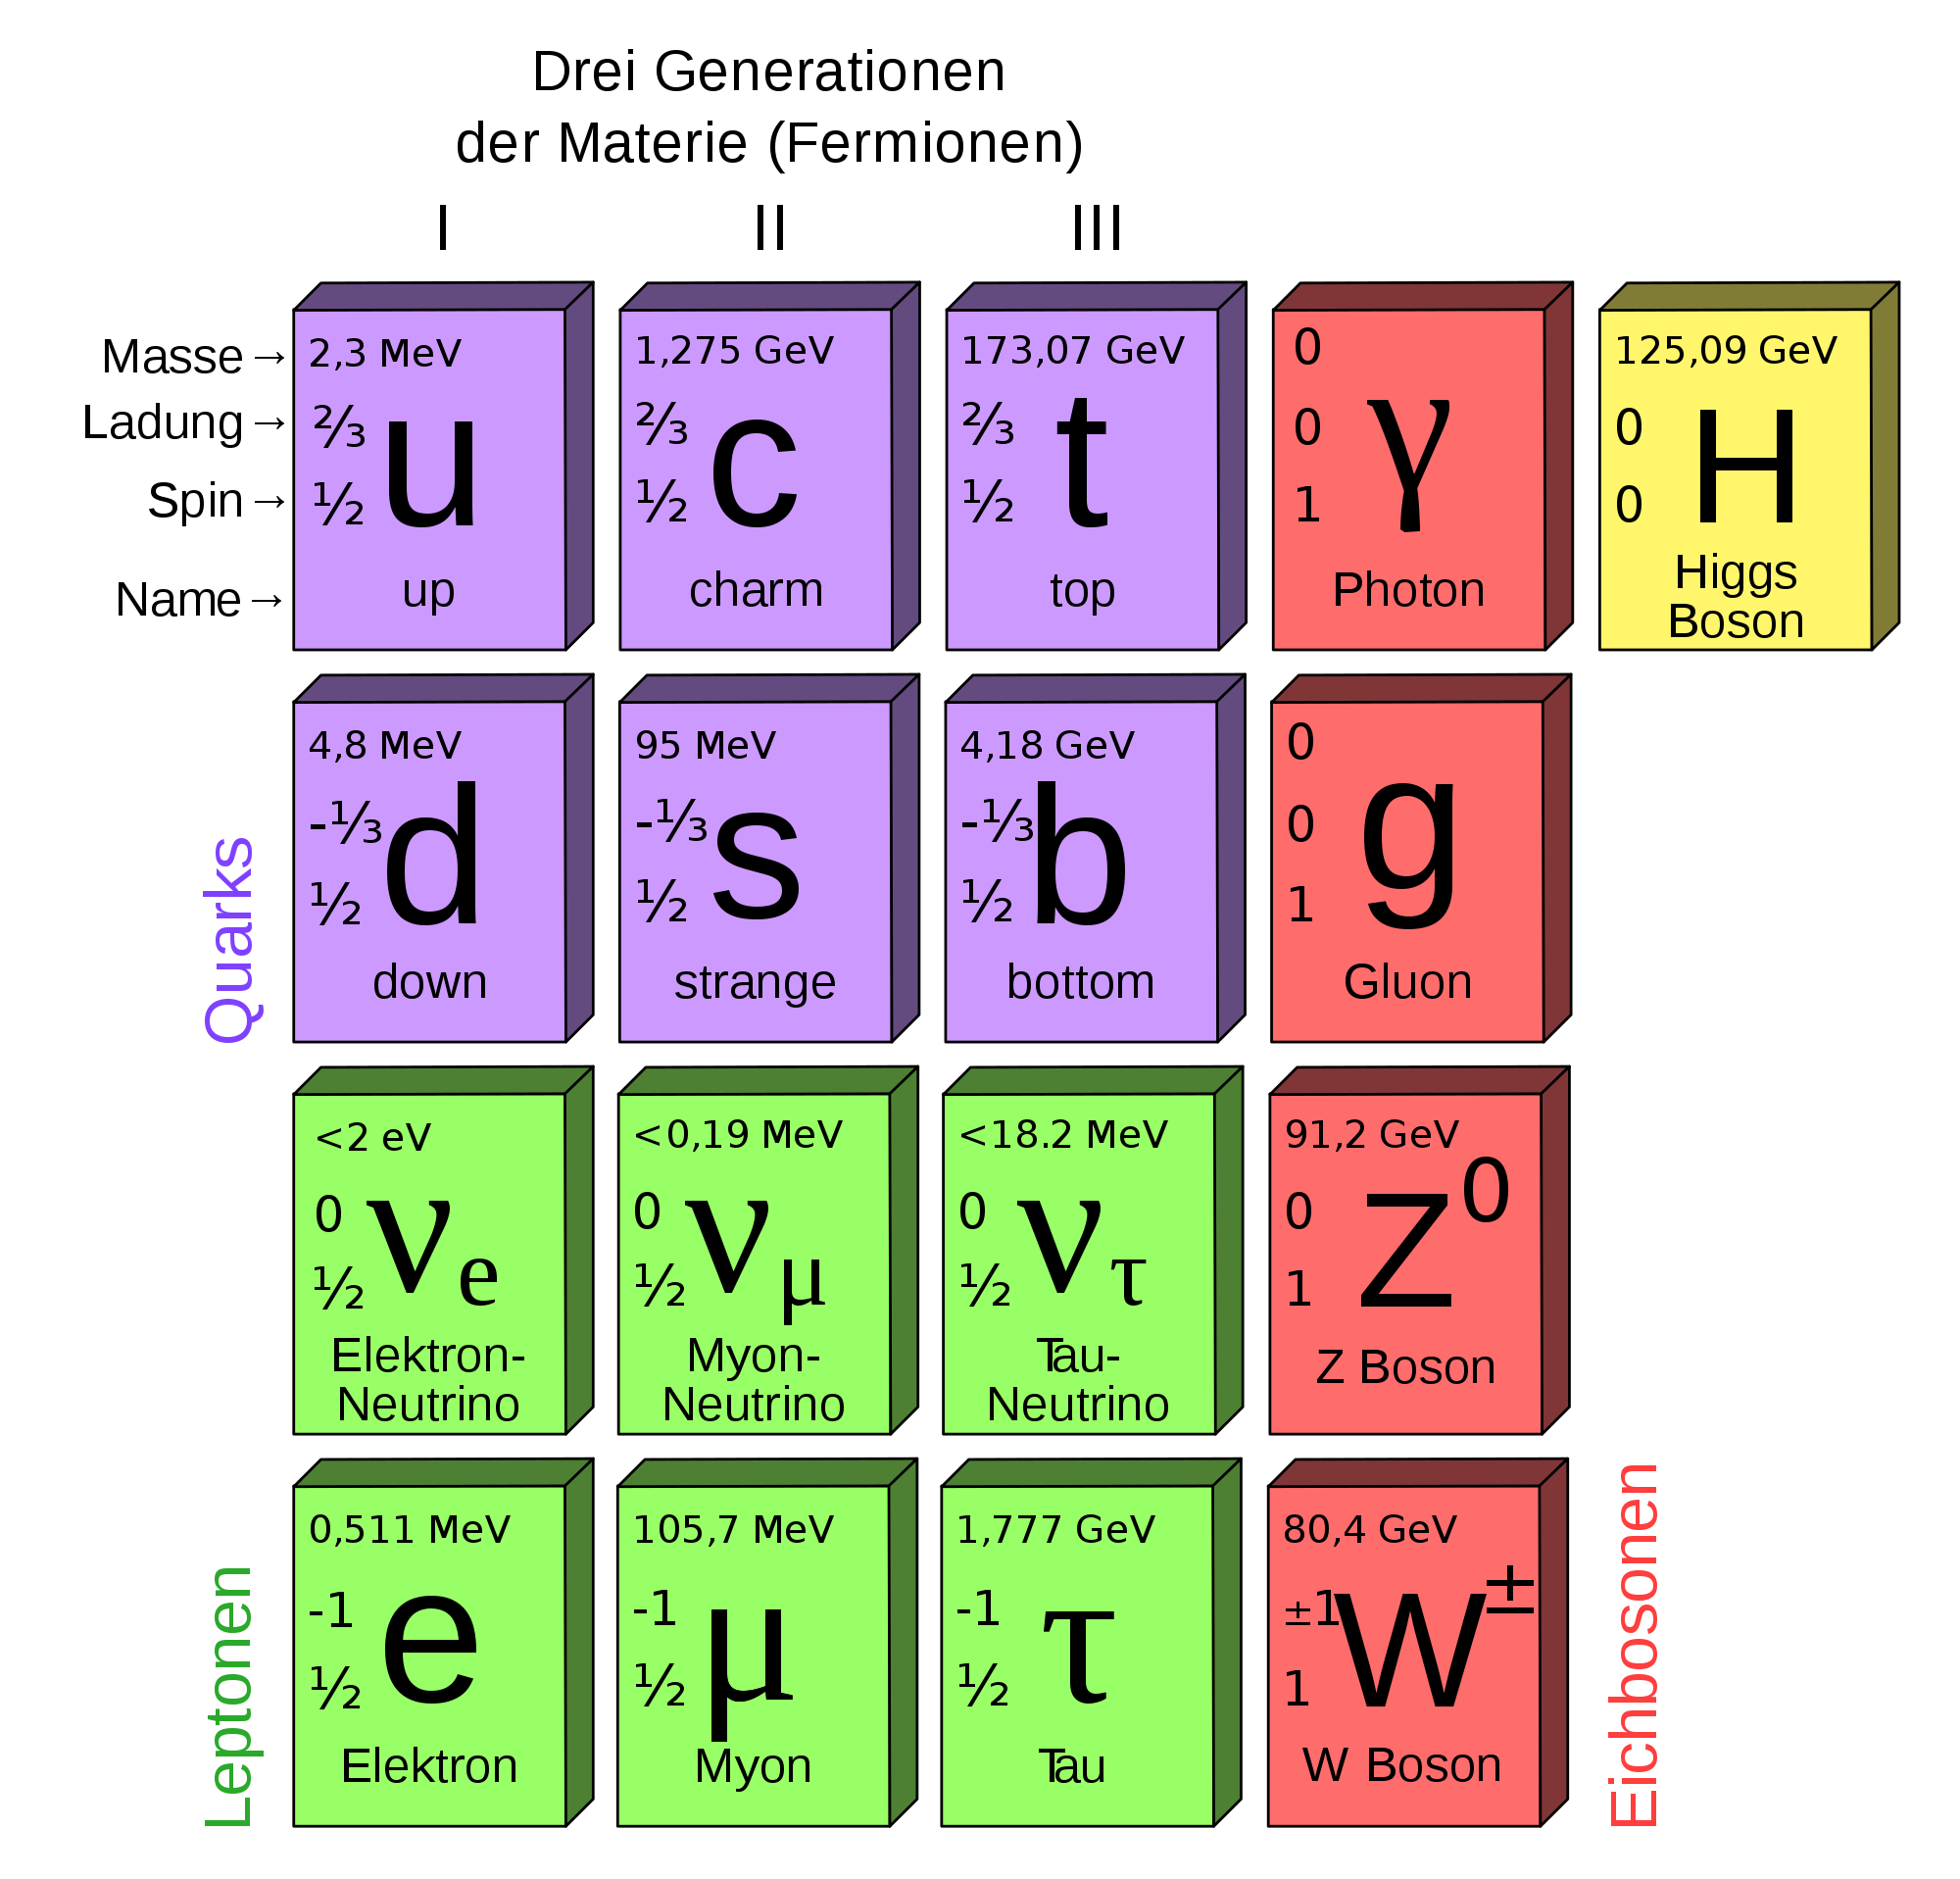
\includegraphics[width=\textwidth]{images/standard_model.png}
        \caption{Standardmodell der Teilchenphysik \cite{standard_model}}
        % \label{}
      \end{figure}
    \end{column}
    \begin{column}{0.4\textwidth}
      \begin{itemize}
        \item Eichboson \rightarrow Elementarteilchen
        \item vermittelt in der elektroschwachen Theorie die geladenen Ströme
        \item Ladung: $q = \pm e$
        \item Spin: $s = 1$
        \item mittlere Lebensdauer: $\SI{3e-25}{\s}$
        \item Masse: $m_W = \SI{80.379(12)}{\GeV}$
      \end{itemize}
    \end{column}
  \end{columns}
\end{frame}

\subsection{Entdeckung des W-Bosons}
\begin{frame}{Entdeckung des W-Bosons}
  \begin{columns}
    \begin{column}{0.4\textwidth}
      \begin{figure}
        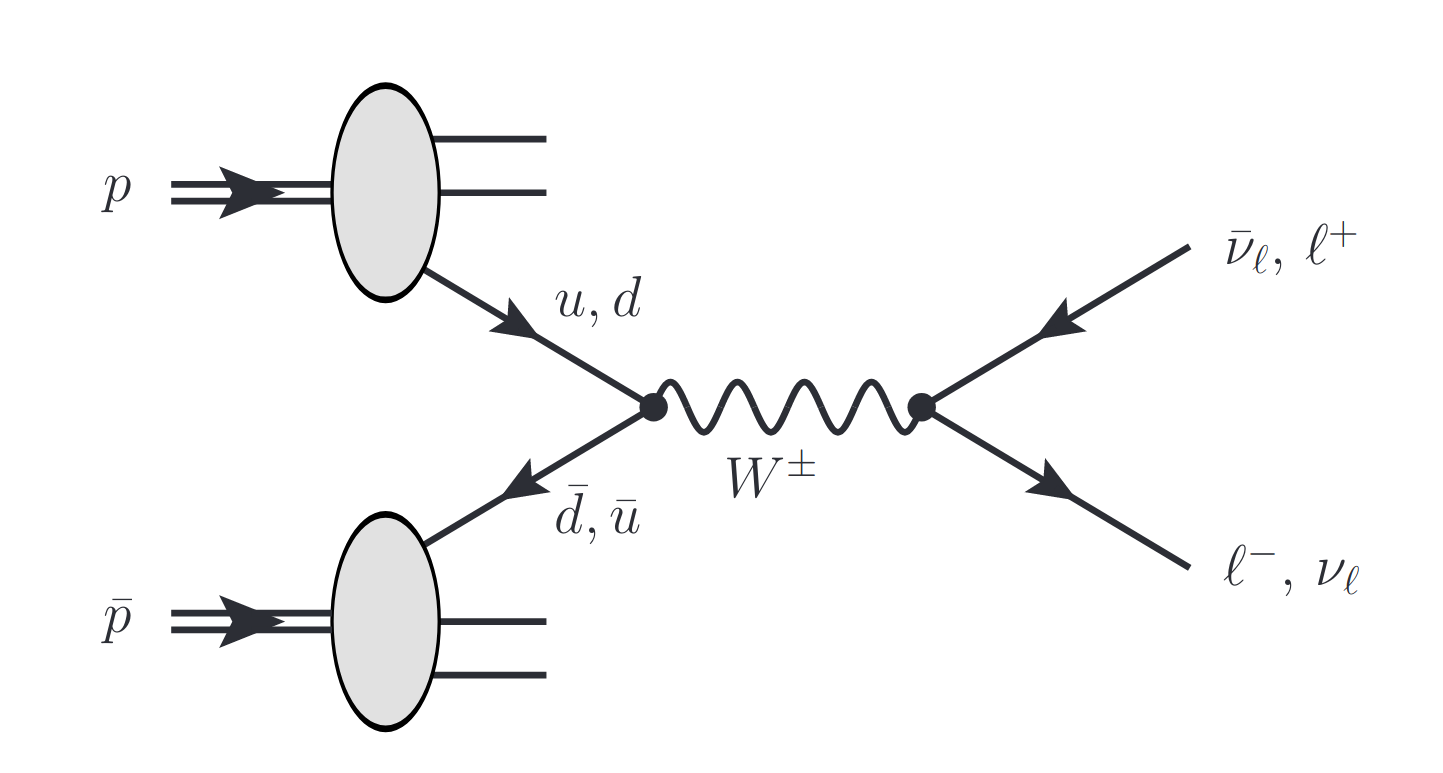
\includegraphics[width=\textwidth]{images/feynman.png}
        \caption{Feynman-Diagramm niedrigster Ordnung zur Erzeugung von W-Bosonen \cite{skript}}
        \label{fig:feynman}
      \end{figure}
    \end{column}
    \begin{column}{0.4\textwidth}
      \begin{itemize}
        \item 1983 am Super Proton Synchrotron (SPS)
        \item Im naiven Partonmodell entsteht das W-Boson bei Kollision eines Valenzquarks des Protons $(\quarku, \quarkd)$ mit einem Valenzantiquark des Antiprotons $(\antiquarku, \antiquarkd)$
        % \item Valenzquark und -antiquark tragen je einen Impulsanteil von $x_{1,2} \approx \SI{0,2}{}$ des (Anti-)Protons
        % \item Benötigte Parton-Parton-Schwerpunktsenergie $\sqrt{\hat{s}} = \SI{80}{\GeV}$ \rightarrow benötigte $\proton \antiproton$-Schwerpunktsenergie $\sqrt{s} = \sqrt{\frac{\hat{s}}{x_1 x_2}} \approx \SI{400}{\GeV}$
      \end{itemize}
    \end{column}
  \end{columns}



\end{frame}

\begin{frame}
  \begin{itemize}
    \item Valenzquark und -antiquark tragen je einen Impulsanteil von $x_{1,2} \approx \SI{0,2}{}$ des (Anti-)Protons
    \item Um ein W-Boson zu erzeugen, wird eine Parton-Parton-Schwerpunktsenergie von $\sqrt{\hat{s}} = \SI{80}{\GeV}$ und somit eine $p \bar{p}$-Schwerpunktsenergie von $\sqrt{s} = \sqrt{\frac{\hat{s}}{x_1 x_2}} \approx \SI{400}{\GeV}$ benötigt
    \item Solche Schwerpunktsenergien waren zuerst am SPS vorhanden ($\sqrt{s} = \SI{540}{\GeV}$)
  \end{itemize}
\end{frame}

\subsection{Motivation}
\begin{frame}{Motivation}
  \begin{itemize}
    \item W- und Z-Masse bestimmen zusammen den schwachen Mischungswinkel
    \item durch genaue Kenntnis der W- und t-Masse lässt sich die Masse des Higgs-Bosons eingrenzen
  \end{itemize}
\end{frame}

\subsection{Theoretische Grundlagen}
\begin{frame}{Theoretische Grundlagen}
   \begin{itemize}
     \item Im Gegensatz zum Z-Nachweis im Zerfall $Z \rightarrow \ell^+ \ell^-$ über die invariante Masse des Leptonpaares kann man hier die Vierervektoren der Zerfallsprodukte nicht vollstandig bestimmen
     \item longitudinaler Impuls $p_z$ des Schwerpunktsystems der Kollision ist, weil das System geboostet ist, nicht bekannt \\
     \item[$\longrightarrow$] Lösung: Verwendung transversaler Größen
   \end{itemize}
\end{frame}

\begin{frame}
  \begin{itemize}
    \item im Zerfall $W \rightarrow \ell \nu$ insbesondere die Transversalimpulse des Leptons $p^\ell_T$ und des Neutrinos $p^\nu_T$ von besonderem Interesse
    \item Der Transversalimpuls des Neutrinos kann nur indirekt über "fehlende transversale Energie"  $\cancel{\it{E}}_{T}$ bestimmt werden
    \item Wenn man annimmt, dass das Neutrino das einzige Teilchen ist, das undetektiert dem Detektor entkommt, kann man ̈uber die Erhaltung des Transversalimpulses $\sum \vec{p}_T$ die transversale Flugrichtung und Energie des Neutrinos bestimmen.
  \end{itemize}
\end{frame}

\begin{frame}
  \begin{itemize}
    \item eine weitere Observable ist die "transversale Masse" $m_T$
    \begin{equation*}
      m_T = 2 p^\ell_T p^\nu_T \left(1 - \cos{\left(\varphi^\ell-\varphi^\nu \right)} \right)
    \end{equation*}
    \begin{center}
      \small{$p^\nu_T = \cancel{\it{E}}_{T}$, $\varphi^\ell-\varphi^\nu \: \hat{=} \: \text{Öffnungswinkel zwischen den Transversalimpulsen des Leptons und des Neutrinos}$}
    \end{center}
    \item Im Ruhesystem des W-Bosons und unter Annahme einer verschwindenden Zerfallsbreite $\Gamma_W$ ist $p_T = \frac{m_W}{2} \sin{(\theta)}$, und somit
    \begin{equation*}
      m_T = m_W \sin{(\theta)}
    \end{equation*}
    \item Der differenzielle Wirkungsquerschnitt als Funktion von $m_T$ wird durch eine Variablentransformation $\mu = \frac{m_T}{m_W} = \sin{(\theta)}$ im Wirkungsquerschnitt gewonnen
    \begin{equation*}
      \frac{\symup{d}\sigma}{\symup{d}\mu} = \frac{\symup{d} \sigma}{\symup{d} \cos{\theta}} \left| \frac{\symup{d} \cos{(\theta)}}{\symup{d} \mu} \right|
    \end{equation*}
  \end{itemize}
\end{frame}

\begin{frame}
  \begin{columns}
    \begin{column}{0.5\textwidth}
      \begin{figure}
        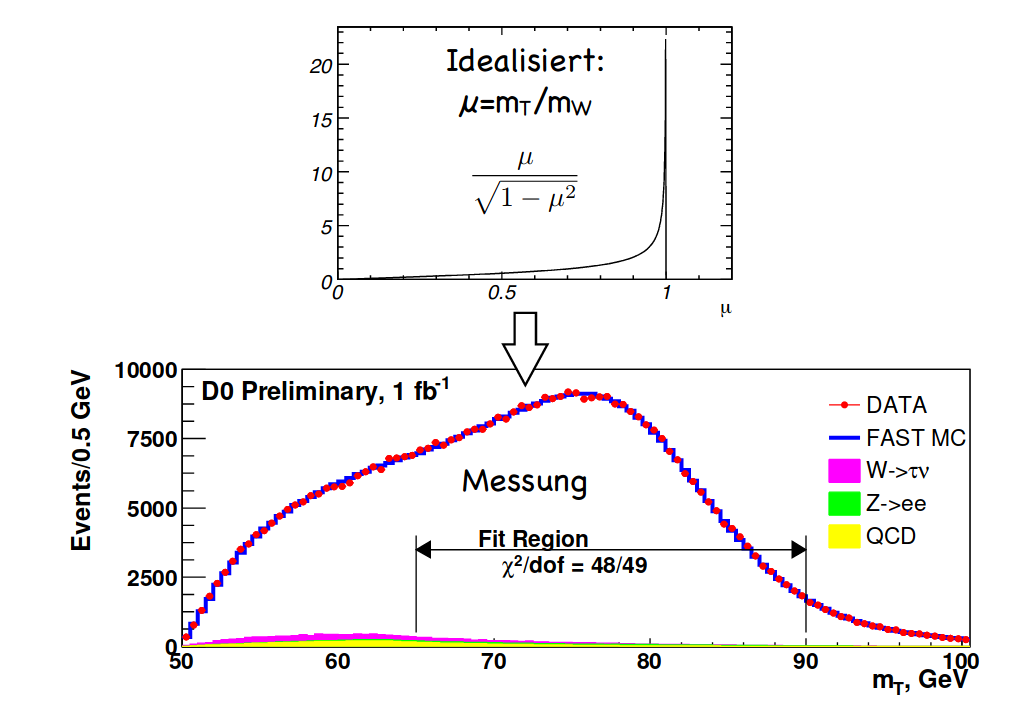
\includegraphics[width=\textwidth]{images/jacobi-peak.png}
        \caption{Darstellung der Jacobi-Kante in idealisierter Form und im Experiment \cite{vorlesung}.}
        % \label{}
      \end{figure}
    \end{column}
    \begin{column}{0.4\textwidth}
      \begin{itemize}
        \item Man erhält für die Jacobi-Determinante dieser Variablentransformation
        \begin{equation*}
          \frac{\symup{d} \cos{(\theta)}}{\symup{d} \mu} = \frac{\symup{d}}{\symup{d}\mu} \sqrt{1-\mu^2} = - \frac{\mu}{\sqrt{1-\mu^2}}
        \end{equation*}
        \item Der differenzielle Wirkungsquerschnitt als Funktion von $m_T$ besitzt damit einen scharfen Knick bei $m_T = m_W$ , den man als "Jacobi-Kante" bezeichnet
      \end{itemize}
    \end{column}
  \end{columns}
\end{frame}

\begin{frame}
  \begin{itemize}
    \item Eine Jacobi-Kante tritt analog auch im differenziellen Wirkungsquerschnitt $\frac{\symup{d} \sigma}{\symup{d} p_T}$ bei einem Transversalimpuls von $p_T = \sfrac{m_w}{2}$ auf
    \item Im Experiment ist Jacobi-Kante verschmiert
    \begin{itemize}
      \item[\rightarrow] W-Boson wird i.A. nicht in Ruhe erzeugt
      \item[\rightarrow] W-Boson besitzt endliche Zerfallsbreite
      \item[\rightarrow] Detektorauflösung
      \item[\rightarrow] Unsicherheiten in der Rekonstruktion
    \end{itemize}
  \end{itemize}
\end{frame}

\section{Tevatron}

\subsection{Allgemeines}

\begin{frame}{Allgemeines}
    \begin{itemize}
      \item Betrieb durch das Fermilab (Batavia, Illinois)
      \item Proton-Antiproton-Beschleuniger
      \item der sträkste Beschleuniger nach dem LHC am CERN
      \item Umfang: $\SI{6}{\km}$
      \item Schwerpunktsenergie: $\SI{1,96}{\TeV}$
      \item 1994-1995: integrierte Luminosität von $\SI{100}{\pico \barn ^{-1}}$
      \item stillgelegt seit $29.09.2011$
    \end{itemize}
\end{frame}

% Duringthe 1994–1995 running period, the accelerator reached apeak luminosity of 2.5×1031cm−2s−1and delivered anintegrated luminosity of about 100 pb−1.

\subsection{Beschleuniger-Kette}

\begin{frame}
  \begin{figure}
    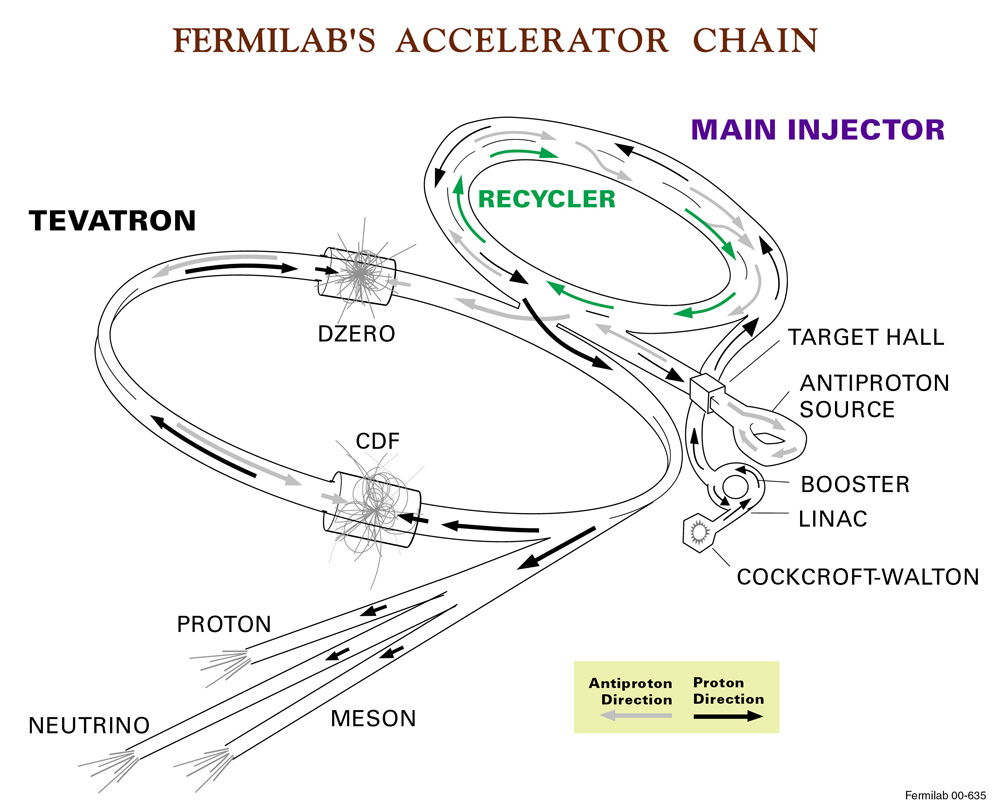
\includegraphics[width=0.55\textwidth]{images/accelerator_chain.jpg}
    \caption{Beschleuniger-Kette am Fermilab \cite{accelerator_chain}.}
    % \label{}
  \end{figure}
\end{frame}

\subsection{Detektoren}

\subsubsection{CDF}

\begin{frame}{CDF}
    \begin{figure}
      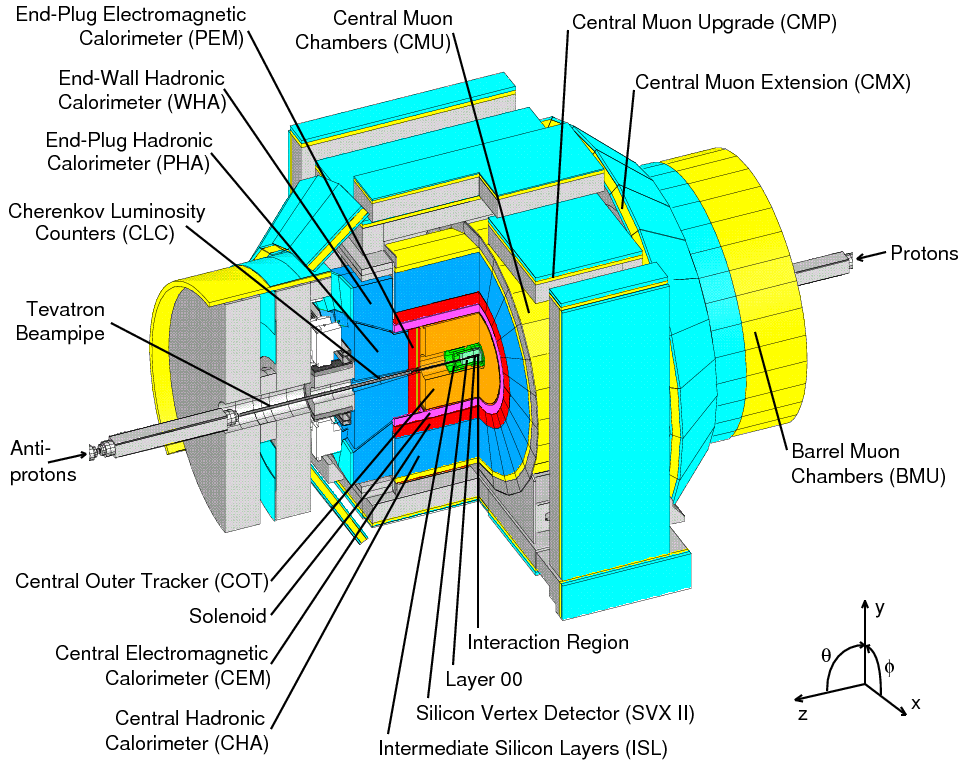
\includegraphics[width=0.55\textwidth]{images/CDF.png}
      \caption{Schematischer Aufbau des CDF-Detektors \cite{CDF_aufbau}}
      % \label{}
    \end{figure}
\end{frame}


\subsubsection{D0}

\begin{frame}{D0}
  \begin{figure}
    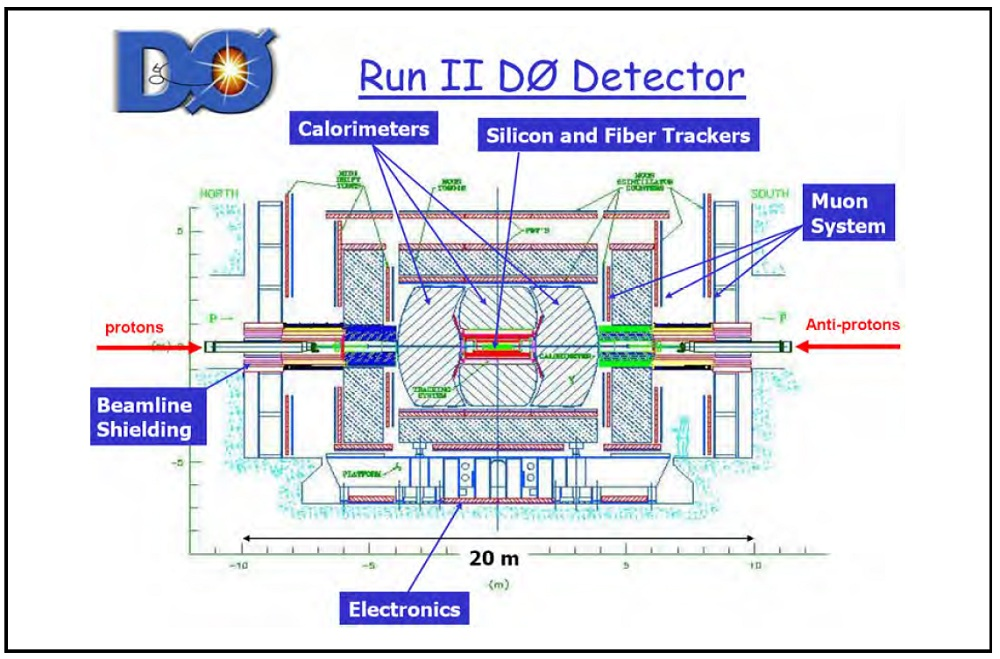
\includegraphics[width=0.65\textwidth]{images/d0.jpg}
    \caption{Schematischer Aufbau des D0-Detektors \cite{D0}}
    % \label{}
  \end{figure}
\end{frame}

\section{Messstrategie}

\subsection{Event Generation}

\begin{frame}{}

\end{frame}

\subsection{Track Momentum Calibration}

\begin{frame}{}

\end{frame}

\subsection{Calorimeter Energy Calibration}

\begin{frame}{}

\end{frame}

\subsection{Hadronic Recoil Measurement and Simulation}

\begin{frame}{}

\end{frame}

\subsection{Backgrounds}

\begin{frame}{}

\end{frame}

\subsection{Mass Fit and Systematics}

\begin{frame}{}

\end{frame}

\begin{frame}{Zusammenfassung}
  \begin{figure}
    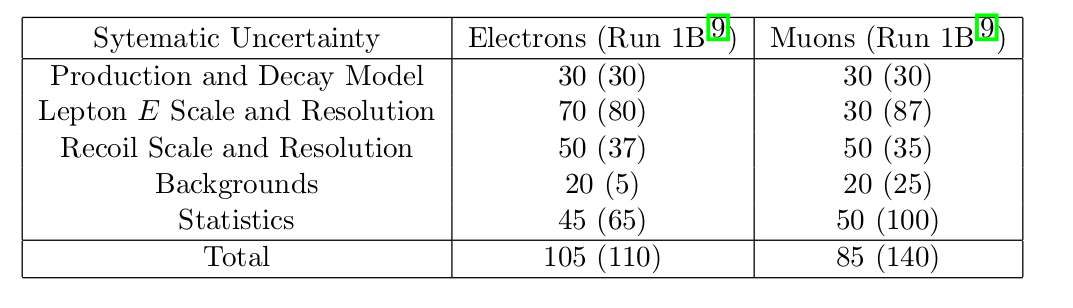
\includegraphics[width=\textwidth]{images/unsicherheiten.png}
    \caption{Unsicherheiten der W-Massenmessung in $\frac{\si{\MeV}}{c^2}$ bei der Nutzung von $\SI{0,2}{\femto \barn^{-1}}$ von CDF Run 2 Daten. In Klammern sind die Unsicherheiten aus CDF Run 1B.}
    % \label{}
  \end{figure}
\end{frame}




% \begin{frame}{Transversale Größen}
 % \begin{columns}
   % \begin{column}{0.4\textwidth}
     % Text,    der    in    der    ersten    Spalte    steht
   % \end{column}
   % \begin{column}{0.4\textwidth}
     % Text,    der    in    der    zweiten    Spalte    steht
   % \end{column}
 % \end{columns}
% \end{frame}

% \section{Test}
%
% \begin{frame}
  % \begin{beamercolorbox}[center, wd=\textwidth]{titlegraphic}
    % 
\includegraphics[width=0.3\textwidth]{images/particle_zoo.jpg}
  % \end{beamercolorbox}%
% \end{frame}

\section{Literatur}
\begin{frame}[allowframebreaks]{Literatur}
  \printbibliography
\end{frame}

\end{document}
